\chapter{Степени, экспонента и логарифмы}\label{chap:c14-exponential}\markright{Глава 22}
\begin{definition}\term{Степенная функция} (\emph{power function}) — функция \(y = x^{r}\) с фиксированным показателем \(r\); допустимые \(x\) зависят от показателя.\end{definition}
\begin{definition}\term{Показательная функция} (\emph{exponential function}) — \(y = a^{x}\) при \(a > 0\) и \(a \ne  1;\allowbreak x\) может быть любым действительным числом.\end{definition}
\begin{definition}\term{Логарифм} (\emph{logarithm}) \(\log _{a} b\) — показатель степени, в которую нужно возвести \(a\), чтобы получить \(b\): \(a^{c} = b\) означает \(\log _{a} b = c\).\end{definition}
Условия логарифма: \(a > 0,\allowbreak a \ne  1,\allowbreak b > 0\).\par
\section{Свойства показательной и логарифмической функций}
\(a^{x}\) всегда положительно. При \(a > 1\) функция возрастает, при \(0 < a < 1\) убывает. Логарифм с тем же основанием меняется в том же направлении.\par
\(\log _{a} 1 = 0;\allowbreak \log _{a} a = 1\). При допустимых значениях \(\log _{a} (a^{x}) = x\) и \(a^{\log _{a} b} = b\).\par
При \(u,\allowbreak v > 0\): \(\log _{a} (uv) = \log _{a} u + \log _{a} v;\allowbreak \log _{a} (\frac{u}{v}) = \log _{a} u - \log _{a} v\).\par
При \(u > 0\): \(\log _{a} (u^{r}) = r \log _{a} u\). Формула смены основания: \(\log _{a} u = \frac{\log _{c} u}{\log _{c} a}\) при \(c > 0,\allowbreak c \ne  1\).\par
Графики \(y = a^{x}\) и \(y = \log _{a} x\) симметричны относительно прямой \(y = x\).\par
\section{Две важные степенные функции}
\(y = \frac{1}{x}\): \(x \ne 0\), значения \(y \ne  0\). \(y = \sqrt{x}\): \(x \ge 0\), значения \(y \ge  0\).\par
{\small\textit{Пример: \(\log _{2} 8 = 3\), потому что \(2^{3} = 8\). Неравенство \((\frac{1}{2})^{x} > (\frac{1}{2})^{3}\) даёт \(x < 3\).}}\par

\section{Число \(e\), натуральный логарифм и экспонента}
\par\addvspace{5pt}\begin{lrbox}{\CatFlowBox}\begin{minipage}[t]{\linewidth}
\setlength{\parskip}{5pt}\setlength{\columnsep}{4.5mm}\setlength{\intextsep}{0pt}
\begin{wrapfigure}[11]{l}{54mm}

\includegraphics[width=54mm,height=58mm,keepaspectratio]{images/unique/art-193.png}
\label{catflow:193}
\end{wrapfigure}
Рассмотрим учебную модель: на счёте \(1\) условная денежная единица, годовая ставка равна \(100\%\). Если проценты начисляют один раз в конце года, получается \(2\). Если год делят на \(n\) равных частей и каждый раз прибавляют \(\frac1n\) текущей суммы, через год получается \(a_n=(1+\frac1n)^n\). Например, \(a_1=2\), \(a_2=2{,}25\), \(a_4=2{,}44140625\). Чем чаще начисление, тем ближе итог к определённому числу; он не растёт без границ.
\par\WFclear\end{minipage}\end{lrbox}%
\ifdim\dimexpr\ht\CatFlowBox+\dp\CatFlowBox\relax<64mm\dp\CatFlowBox=\dimexpr64mm-\ht\CatFlowBox\relax\fi%
\noindent\usebox{\CatFlowBox}\par\addvspace{5pt}
\begin{definition}\term{Число \(e\)} (\emph{Euler's number}) — стандартная положительная константа \(e\approx2{,}718281828\). Её точное определение как предела \((1+1/n)^n\) и доказательство существования даны в подразделе \ref{sec:e-construction}.\end{definition}
\begin{definition}\term{Экспонента} (exponential function) — функция \(\exp x=e^x\), определённая для всех \(x\in\mathbb R\). Её значения положительны, и она строго возрастает.\end{definition}
\begin{definition}\term{Натуральный логарифм} (natural logarithm) — логарифм по основанию \(e\): \(\ln x=\log_e x\) при \(x>0\). Он является обратной функцией к экспоненте.\end{definition}
По определениям \(\ln1=0\), \(\ln e=1\), \(\ln(e^x)=x\) для всех действительных \(x\), а \(e^{\ln x}=x\) для \(x>0\). Сохраняются правила \(e^{x+y}=e^xe^y\) и \(\ln(uv)=\ln u+\ln v\) при \(u,v>0\).
\begin{theorem}[Переход к натуральному основанию]\label{thm:legacy-c14-2}
При \(a>0\), \(a\ne1\), \(u>0\) выполнено \(\log_a u=\frac{\ln u}{\ln a}\). Для \(a>0\) и \(x\in\mathbb R\) выполнено \(a^x=e^{x\ln a}\).
\end{theorem}
\begin{proof}
Положим \(r=\log_a u\); тогда \(u=a^r\). По правилу логарифма степени \(\ln u=r\ln a\). Поскольку \(a\ne1\), число \(\ln a\ne0\), и деление даёт первую формулу. Далее \(\ln(a^x)=x\ln a\); применив экспоненту к обеим частям, получаем вторую формулу.
\end{proof}
\section{Правила степеней и логарифмов с условиями}
Для \(a,b>0\) и действительных \(r,s\) действуют
\[
a^{r+s}=a^ra^s,\qquad (a^r)^s=a^{rs},\qquad (ab)^r=a^rb^r.
\]
Ограничение на основания существенно: для отрицательного основания произвольная действительная степень может не определяться. При \(a>0\), \(a\ne1\), \(u,v>0\)
\[
\begin{gathered}
\log_a(uv)=\log_a u+\log_a v,\quad
\log_a\frac uv=\log_a u-\log_a v,\\
\log_a(u^r)=r\log_a u.
\end{gathered}
\]
Например, если \(s=\log_a u\), \(t=\log_a v\), то \(uv=a^sa^t=a^{s+t}\), поэтому логарифм произведения равен \(s+t\). Для частного используется \(u\,v^{-1}\), а для степени — \((a^s)^r=a^{sr}\). Равенство \(\log_a(u+v)=\log_a u+\log_a v\) отсюда не следует и в общем случае неверно: при \(a=2,u=v=1\) слева \(1\), справа \(0\).

\par\noindent\begin{minipage}{\linewidth}\section*{Графики}
\begin{center}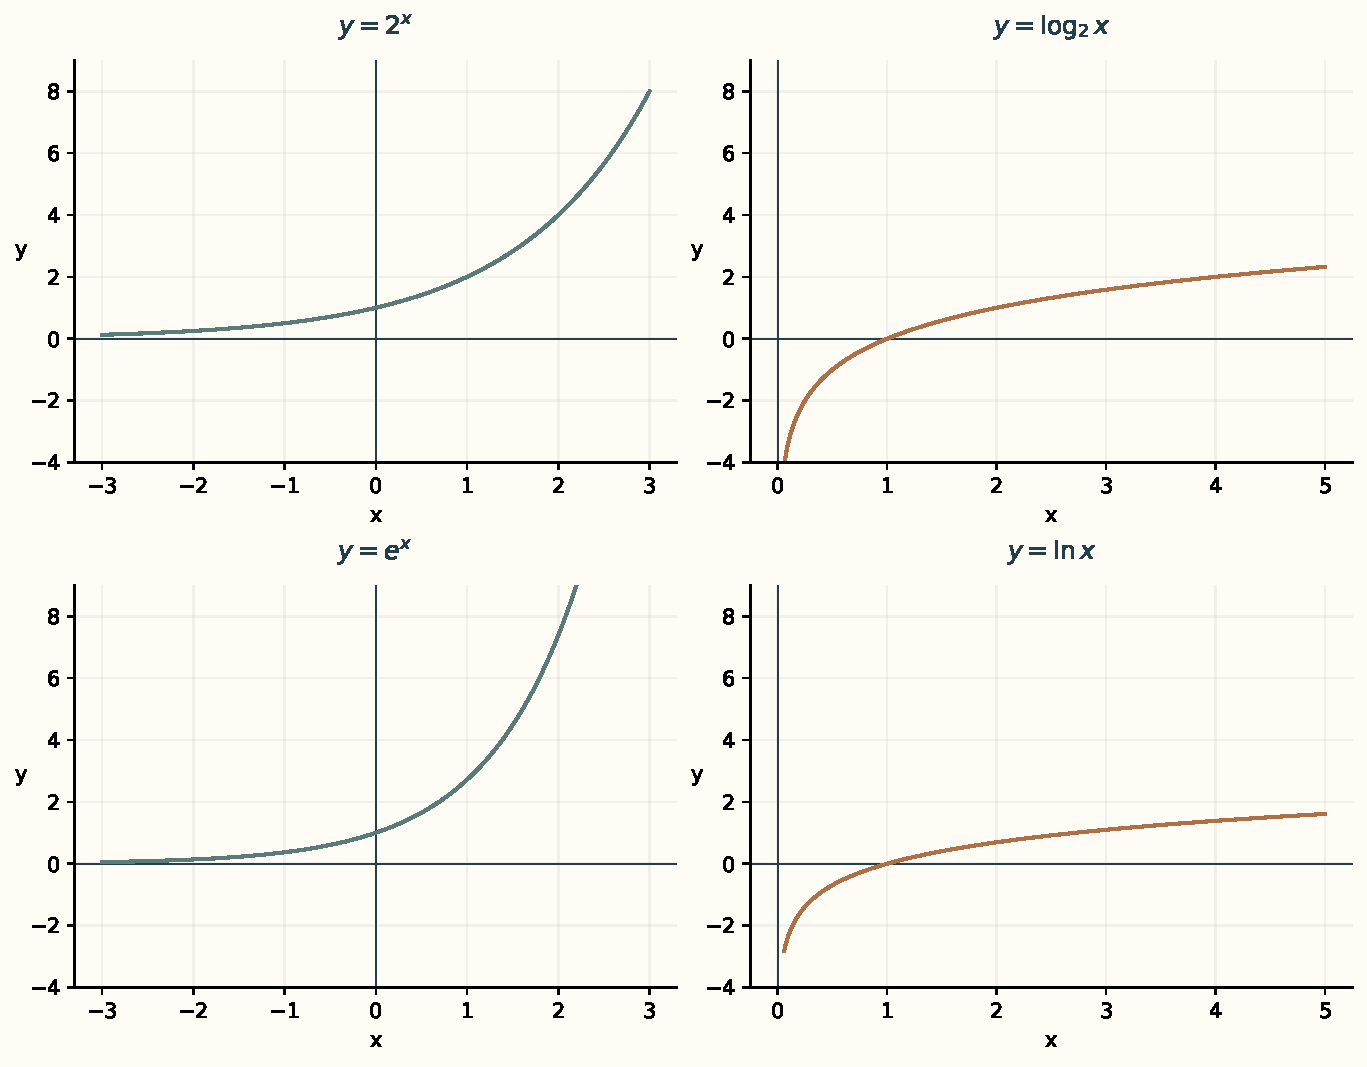
\includegraphics[width=\textwidth,height=.79\textheight,keepaspectratio]{images/atlas-exponential-basic.pdf}\par\small Показательные и логарифмические функции\end{center}\end{minipage}\par
\Needspace{7\baselineskip}\section*{Задачи}
\begingroup\setlength{\parskip}{2pt}
\noindent\begin{minipage}[t]{\linewidth}\textbf{22.1.} Построй \(y = \dfrac{1}{x}\). Укажи область определения и область значений.\par\end{minipage}\par
\noindent\begin{minipage}[t]{\linewidth}\textbf{22.2.} Построй \(y = \sqrt{x}\). Укажи область определения и область значений.\par\end{minipage}\par
\noindent\begin{minipage}[t]{\linewidth}\textbf{22.3.} Реши \(x^{3} = - 27\).\par\end{minipage}\par
\noindent\begin{minipage}[t]{\linewidth}\textbf{22.4.} Реши \(2^{x} = 32\).\par\end{minipage}\par
\noindent\begin{minipage}[t]{\linewidth}\textbf{22.5.} Реши \(3^{x - 1} = 9\).\par\end{minipage}\par
\par\addvspace{5pt}\begin{lrbox}{\CatFlowBox}\begin{minipage}[t]{\linewidth}
\setlength{\parskip}{5pt}\setlength{\columnsep}{4.5mm}\setlength{\intextsep}{0pt}
\begin{wrapfigure}[12]{l}{54mm}

\includegraphics[width=54mm,height=58mm,keepaspectratio]{images/unique/art-40.png}
\label{catflow:40}
\end{wrapfigure}
\textbf{22.6.} Реши \((\dfrac{1}{2})^{x} > \dfrac{1}{8}\).\par

\textbf{22.7.} Вычисли \(\log _{2} 8 + \log _{3} 1\).\par

\textbf{22.8.} Вычисли \(\log _{5} (\dfrac{1}{25})\).\par

\textbf{22.9.} Реши \(\log _{2} (x - 1) = 3\).\par

\textbf{22.10.} Найди область определения \(y = \log _{3} (5 - x)\).\par

\textbf{22.11.} При \(a > 0\) упрости \(\log _{2} (8 a) - \log _{2} a\).\par

\textbf{22.12.} Сравни \(2^{0{,}3}\) и \(2^{0{,}7}\); затем \((\dfrac{1}{3})^{0{,}3}\) и \((\dfrac{1}{3})^{0{,}7}\).\par
\par\WFclear\end{minipage}\end{lrbox}%
\ifdim\dimexpr\ht\CatFlowBox+\dp\CatFlowBox\relax<64mm\dp\CatFlowBox=\dimexpr64mm-\ht\CatFlowBox\relax\fi%
\noindent\usebox{\CatFlowBox}\par\addvspace{5pt}

\noindent\begin{minipage}[t]{\linewidth}\textbf{22.13.} В учебной модели стоимость оборудования каждый год уменьшается вдвое: \(S (t) = 80000 \cdot  (\dfrac{1}{2})^{t}\) рублей. Найди стоимость через \(3\) года.\par\end{minipage}\par
\noindent\begin{minipage}[t]{\linewidth}\textbf{22.14.} Модель роста культуры: \(N (t) = 500 \cdot  2^{t}\), где \(t\) — число часов. Через сколько часов станет \(8000\) клеток?\par\end{minipage}\par
\noindent\begin{minipage}[t]{\linewidth}\textbf{22.15.} Для двоичного поиска в массиве из \(2^{k}\) элементов используют модель из \(k\) шагов. Сколько шагов даёт эта модель для \(1024\) элементов?\par\end{minipage}\par
\noindent\begin{minipage}[t]{\linewidth}\textbf{22.16.}\starmark{} Реши \(4^{x} - 5 \cdot  2^{x} + 4 = 0\).\par\end{minipage}\par
\noindent\begin{minipage}[t]{\linewidth}\textbf{22.17.}\starmark{} Реши \(\log _{2} (x - 1) + \log _{2} (x + 1) = 3\).\par\end{minipage}\par
\noindent\begin{minipage}[t]{\linewidth}\textbf{22.18.}\starmark{} Вклад в учебной модели ежегодно увеличивается на \(10 \%\) без пополнений и снятий. Найди наименьшее целое число лет, через которое \(10000\) рублей станут не меньше \(13310\) рублей.\par\end{minipage}\par
\noindent\begin{minipage}[t]{\linewidth}\textbf{22.19.}\starmark{} Докажи, что для \(a,b>0\), \(a\ne1\), \(b\ne1\) выполнено \(\log_a b\cdot\log_b a=1\). Объясни, почему нужны ограничения \(a\ne1\) и \(b\ne1\).\par\end{minipage}\par
\noindent\begin{minipage}[t]{\linewidth}\textbf{22.20.} Вычисли \(\exp0\), \(\ln1\), \(\ln(e^3)\), \(\exp(\ln5)\).\par\end{minipage}\par
\noindent\begin{minipage}[t]{\linewidth}\textbf{22.21.} Реши уравнение \(\ln(x-1)=2\), начав с области допустимых значений.\par\end{minipage}\par
\noindent\begin{minipage}[t]{\linewidth}\textbf{22.22.} Без десятичного приближения найди \(\dfrac{\ln8}{\ln2}\) и \(e^{2\ln3-\ln9}\).\par\end{minipage}\par
\noindent\begin{minipage}[t]{\linewidth}\textbf{22.23.} В учебной модели начальная сумма \(1000\) рублей увеличивается за год в \((1+\dfrac1n)^n\) раза. Найди сумму при \(n=2\) и \(n=4\), округлив до копеек. К какому значению приближаются суммы при неограниченном увеличении \(n\)? Используй \(e\approx2{,}718281828\).\par\end{minipage}\par
\endgroup
